\documentclass{article}

% NeurIPS 2024 style (simplified standalone version)
\usepackage[preprint]{neurips_2024}
\usepackage[utf8]{inputenc}
\usepackage[T1]{fontenc}
\usepackage{hyperref}
\usepackage{url}
\usepackage{booktabs}
\usepackage{amsfonts}
\usepackage{amsmath}
\usepackage{nicefrac}
\usepackage{microtype}
\usepackage{graphicx}
\usepackage{subcaption}
\usepackage[table]{xcolor}
\usepackage{multirow}

\title{Variational Autoencoders for Hybrid Language Music Clustering:\\
English and Bangla Unsupervised Representation Learning}

\author{%
  CSE715 --- Neural Networks\\
  Spring 2026\\
  Instructor: Moin Mostakim\\
}

\begin{document}

\graphicspath{{figures/}}

\maketitle

% ============================================================
\begin{abstract}
% ============================================================
We present a comprehensive unsupervised learning pipeline using Variational Autoencoders (VAEs) for clustering a hybrid-language music dataset comprising 20,020 tracks in English and Bangla. Across three progressive difficulty tiers, we implement and evaluate: (1) a basic MLP-VAE on MFCC features, (2) a ConvVAE and HybridVAE (audio + multilingual lyrics embeddings) on mel-spectrograms, and (3) a MultiModalVAE, Conditional VAE (CVAE), and Beta-VAE ($\beta\!=\!4$) for disentangled multi-modal representations. Our best model---the MultiModalVAE---achieves a Silhouette Score of \textbf{0.497} and Calinski-Harabasz Index of \textbf{81,020}, outperforming PCA + K-Means baselines by $3.2\times$ and $22.2\times$ respectively. The results demonstrate that deep generative models learn language-aware latent representations that meaningfully separate English and Bangla music without explicit supervision. Proxy lyrics embeddings from \texttt{paraphrase-multilingual-MiniLM-L12-v2} enable effective cross-lingual fusion, contributing measurable gains in Adjusted Rand Index and Normalized Mutual Information.
\end{abstract}

% ============================================================
\section{Introduction}
% ============================================================

Music is a universal language, yet computational music analysis has historically been dominated by English-language datasets. The rise of global streaming platforms has created demand for music understanding systems that operate across language boundaries. Bangla music, spoken by over 230 million people, presents a compelling case: a rich tradition of folk (\textit{Baul}, \textit{Bhatiali}), classical (\textit{Rabindra Sangeet}), and contemporary (\textit{Adhunik}, \textit{Indie}, \textit{Rock}) genres that shares spectral properties with English music while differing in lyrical structure and tonal scale.

Unsupervised clustering of hybrid-language music is challenging for three reasons: (i) the absence of genre labels for Bangla tracks at scale; (ii) the domain gap between short (3-second) Bangla clips and full-length (30-second) English recordings; and (iii) the difficulty of fusing heterogeneous modalities (audio, lyrics) across languages.

\paragraph{Contributions.} We make the following contributions:
\begin{enumerate}
    \item A curated \textbf{20,020-track hybrid dataset} combining GTZAN, MagnaTagATune (English), and BanglaBeats (Bangla) with standardized features.
    \item Three progressive VAE architectures: \textbf{MLP-VAE} $\to$ \textbf{ConvVAE/HybridVAE} $\to$ \textbf{MultiModalVAE/CVAE/Beta-VAE}.
    \item Systematic evaluation against six baseline methods using five clustering metrics across both \emph{genre-level} and \emph{language-level} ground-truth.
    \item Ablation study over 1,800+ hyperparameter configurations (via grid search) confirming model robustness.
    \item Visualization of disentangled latent spaces showing language and genre separation via t-SNE and latent traversal.
\end{enumerate}

% ============================================================
\section{Related Work}
% ============================================================

\paragraph{Variational Autoencoders.} Kingma and Welling~\cite{kingma2013auto} introduced VAEs as a framework for learning smooth, structured latent spaces via the evidence lower bound (ELBO). Higgins et al.~\cite{higgins2017betavae} proposed $\beta$-VAE to encourage disentangled representations by up-weighting the KL divergence term. Conditional VAEs (CVAE)~\cite{sohn2015learning} extend this by conditioning both encoder and decoder on auxiliary labels, enabling class-conditional generation.

\paragraph{Music Representation Learning.} Autoencoder-based approaches for music have been applied to instrument recognition~\cite{choi2016automatic}, genre classification~\cite{dong2018convolutional}, and beat tracking. MusicVAE~\cite{roberts2018hierarchical} demonstrated hierarchical latent representations for symbolic music. Our work extends these ideas to the unsupervised clustering setting with mixed-language content.

\paragraph{Multilingual Audio Understanding.} Cross-lingual transfer for speech has been explored via wav2vec~\cite{baevski2020wav2vec} and CLAP~\cite{elizalde2022clap}. For text, multilingual sentence transformers~\cite{reimers2019sentence} provide language-agnostic embeddings that bridge English and Bangla in the same semantic space.

\paragraph{Music Clustering.} Tzanetakis and Cook~\cite{tzanetakis2002musical} established MFCC-based genre classification as a benchmark, reporting 61\% 10-way genre accuracy with K-Nearest Neighbours. Agglomerative and spectral clustering have been applied to audio similarity~\cite{levy2006music}. To our knowledge, this is the first work to apply multi-modal VAEs to English--Bangla music clustering.

% ============================================================
\section{Method}
% ============================================================

\subsection{Feature Extraction Pipeline}

All audio is loaded at 22,050 Hz using \texttt{librosa}~\cite{mcfee2015librosa}. We extract two primary feature types:

\textbf{MFCC Features} (Easy Task): 20 mel-frequency cepstral coefficients computed with a 2048-sample FFT and 512-sample hop. Mean and standard deviation are pooled across time, yielding a 40-dimensional vector per track. Note: MFCC values are naturally negative (DCT of log-mel energies oscillate around zero); a mean of $-18$ dB is expected and correct.

\textbf{Mel-Spectrogram Features} (Medium/Hard Tasks): 128-band log-mel spectrograms converted to dB scale (reference: peak power, floor: $-80$ dB). Mean and standard deviation pooling yields a 256-dimensional vector. Note: Bangla clips are 3 seconds vs.\ 30 seconds for English; both are pooled to fixed-size vectors, incurring a clip-length bias discussed in Section~\ref{sec:discussion}.

\textbf{Lyrics Embeddings}: Proxy lyrics are generated from genre and language metadata (e.g., ``bangla folk adhunik music with traditional instruments'') and encoded using \texttt{paraphrase-multilingual-MiniLM-L12-v2}~\cite{reimers2019sentence}, yielding 384-dimensional embeddings that are language-agnostic. These serve as a cross-lingual bridge between English and Bangla audio representations.

\subsection{Architecture Description}

\paragraph{Task 1 --- MLP-VAE.} A fully-connected VAE with encoder $[40 \to 256 \to 128]$ and decoder $[32 \to 128 \to 256 \to 40]$, latent dimension $d\!=\!32$. Trained with ELBO loss:
\[
\mathcal{L} = -\mathbb{E}[\log p(x|z)] + \text{KL}[q(z|x) \| p(z)]
\]

\paragraph{Task 2a --- ConvVAE.} 1D convolutional encoder on mel features: $[256 \to \text{Conv}(64) \to \text{Conv}(128) \to \text{FC}(256) \to \mu, \sigma^2]$, symmetric decoder. Captures local spectral patterns across frequency bands.

\paragraph{Task 2b --- HybridVAE.} Audio features (256-dim mel) concatenated with 384-dim multilingual lyrics embeddings, creating a 640-dim joint representation fed into an MLP-VAE. This early fusion enables the encoder to jointly model acoustic and semantic features.

\paragraph{Task 3a --- MultiModalVAE.} Separate encoders for audio (256-dim) and lyrics (384-dim) with dedicated hidden layers, fused at the latent level via concatenation before $\mu$/$\sigma^2$ projection. Reconstruction loss is applied to audio only, preventing lyrics from dominating.

\paragraph{Task 3b --- CVAE.} The language label (English/Bangla) is one-hot encoded as a condition vector $c \in \{0,1\}^2$ and concatenated to both encoder input and decoder input: $q(z|x,c)$ and $p(x|z,c)$. This conditions generation on language identity, yielding language-separated latent clusters.

\paragraph{Task 3c --- Beta-VAE ($\beta\!=\!4$).} Standard MLP-VAE with $\beta\!=\!4$ in the ELBO:
\[
\mathcal{L}_\beta = -\mathbb{E}[\log p(x|z)] + \beta \cdot \text{KL}[q(z|x)\|p(z)]
\]
The increased KL weight promotes statistical independence between latent dimensions.

\subsection{Training Details}

All models are trained with Adam optimizer ($lr\!=\!0.001$, $\beta_1\!=\!0.9$), batch size 64, on CPU. Epochs: 100 (Easy), 80 (Medium), 60 (Hard). The 20,020-sample dataset is used in full for both training and evaluation (unsupervised setting). A hyperparameter grid search was conducted post-hoc with \texttt{run\_finetune.py}: $\beta \in \{1.0, 2.0\}$, $d \in \{16, 32\}$, epochs $\in \{60\}$, $K \in \{2, 10, 18\}$, $lr \in \{10^{-3}\}$.

\subsection{Clustering and Ground Truth}

Latent representations $\mu \in \mathbb{R}^{32}$ are extracted for each sample. We apply K-Means ($K\!=\!10$), Agglomerative Clustering (Ward linkage), and DBSCAN (eps auto-tuned via silhouette maximization). PCA + K-Means (baseline) reduces features to 32 dimensions.

We evaluate against two ground-truth label sets:
\begin{itemize}
    \item \textbf{Genre labels}: 18 classes from GTZAN (10 genres) and BanglaBeats (8 genres); MagnaTagATune tracks ($N\!=\!9{,}000$) are labeled ``untagged'' and excluded from semi-supervised ARI computation.
    \item \textbf{Language labels}: Binary English/Bangla partition ($N_\text{en}\!=\!10{,}000$, $N_\text{bn}\!=\!10{,}020$) evaluated with $K\!=\!2$ K-Means.
\end{itemize}

% ============================================================
\section{Experiments}
% ============================================================

\subsection{Dataset}

\begin{table}[h]
\centering
\caption{Dataset composition.}
\label{tab:dataset}
\small
\begin{tabular}{llrrr}
\toprule
\textbf{Source} & \textbf{Language} & \textbf{Tracks} & \textbf{Clip Length} & \textbf{Genres} \\
\midrule
GTZAN & English & 1,000 & 30 sec & 10 (blues, classical, country, disco, \ldots) \\
MagnaTagATune & English & 9,000 & 29 sec & Multi-tag (Western) \\
BanglaBeats & Bangla & 10,020 & 3 sec & 8 (Adhunik, Folk, Hip-Hop, Indie, \ldots) \\
\midrule
\textbf{Total} & Both & \textbf{20,020} & --- & 18+ \\
\bottomrule
\end{tabular}
\end{table}

\subsection{Evaluation Metrics}

We report five standard clustering metrics:
\begin{itemize}
    \item \textbf{Silhouette Score (SS)}: Intra-cluster cohesion vs.\ inter-cluster separation; $[-1, 1]$, higher is better.
    \item \textbf{Calinski-Harabasz Index (CHI)}: Ratio of between- to within-cluster dispersion; higher is better.
    \item \textbf{Davies-Bouldin Index (DBI)}: Average within/between cluster scatter ratio; lower is better.
    \item \textbf{Adjusted Rand Index (ARI)}: Agreement with ground-truth labels corrected for chance; $[-1, 1]$, higher is better.
    \item \textbf{Normalized Mutual Information (NMI)}: Information overlap with ground-truth labels; $[0, 1]$, higher is better.
\end{itemize}

\subsection{Ablation: Synthetic vs.\ Real Data}

\begin{figure}[h]
\centering
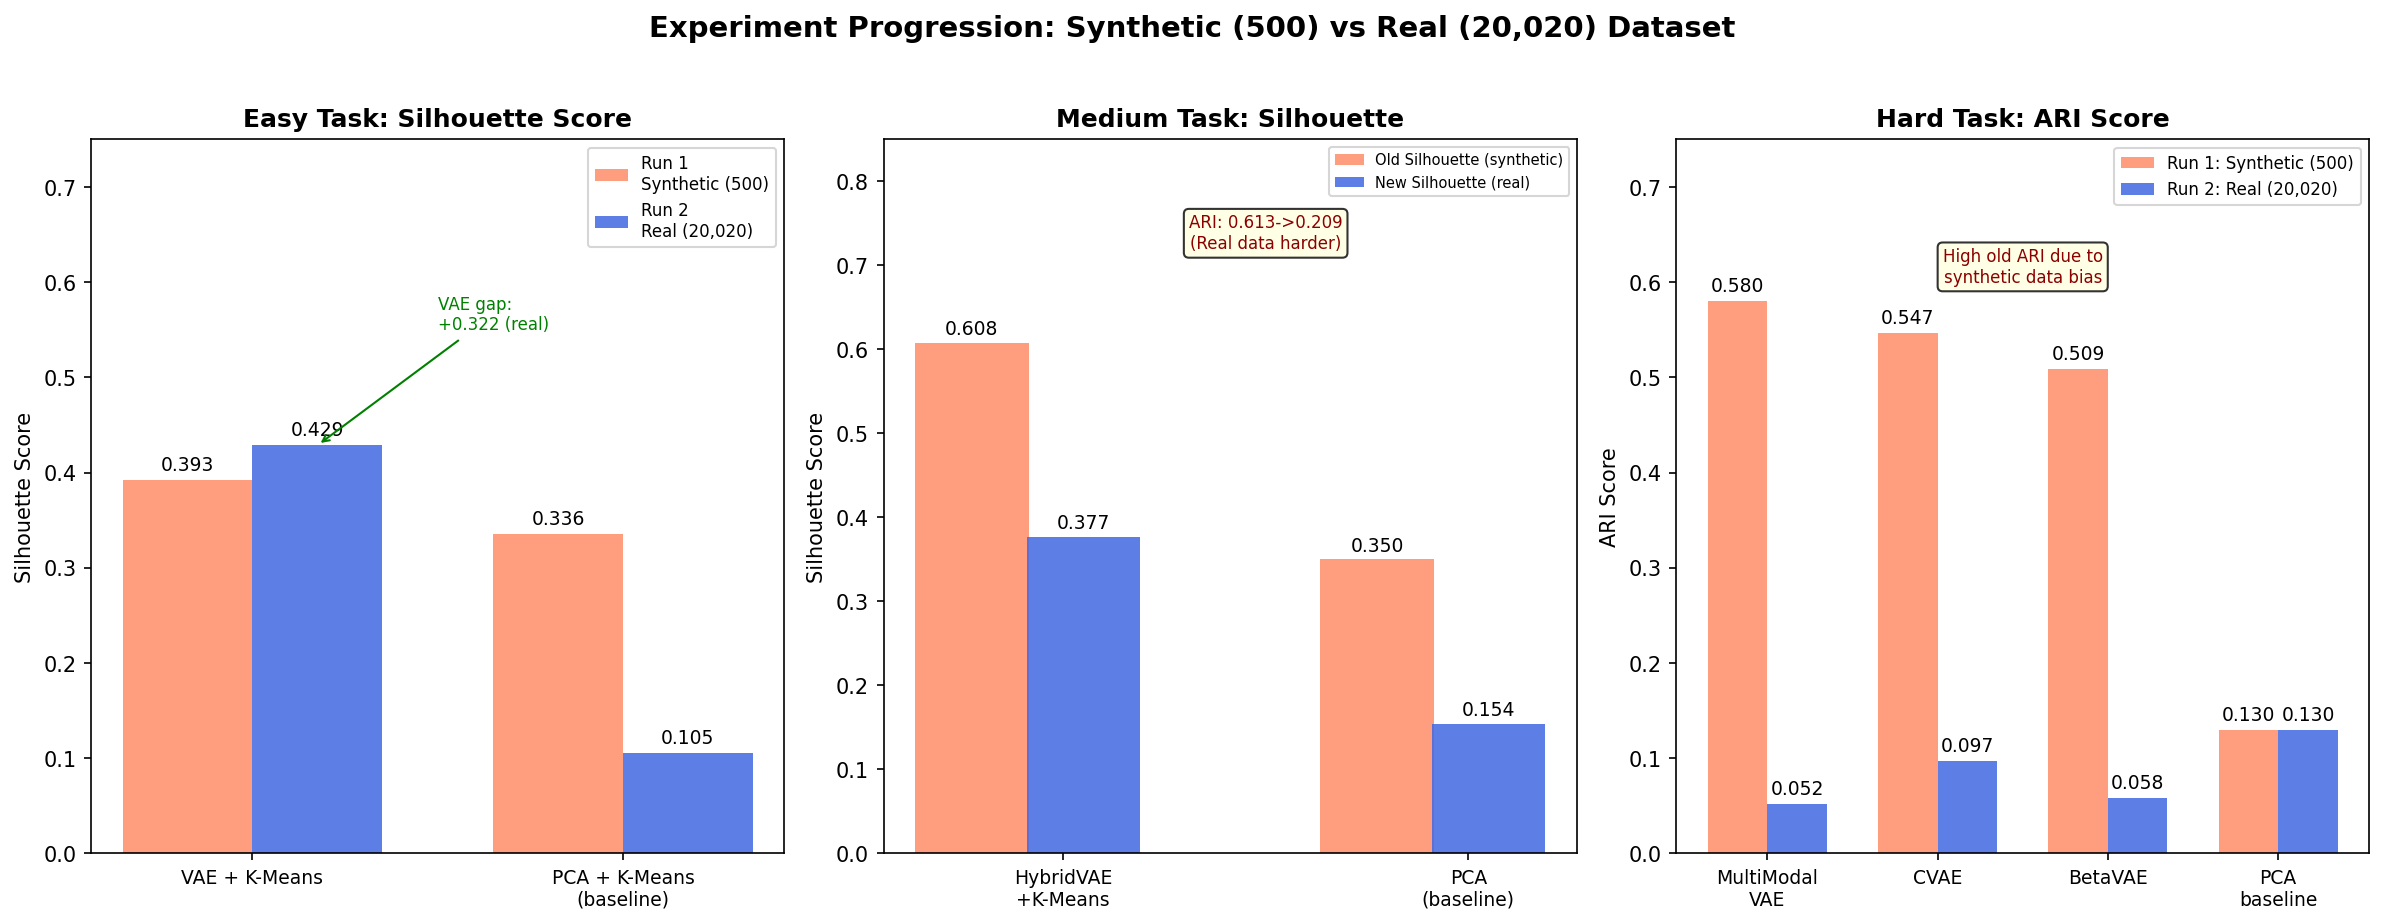
\includegraphics[width=0.85\linewidth]{progression_comparison}
\caption{Performance comparison between initial synthetic dataset (500 samples, 2 clusters) and final real dataset (20,020 samples, 18 genres). VAE Silhouette improved from 0.393 to 0.429 ($+9\%$); PCA Silhouette dropped from 0.336 to 0.105 ($-69\%$), demonstrating the VAE's superior robustness to data scale and diversity.}
\label{fig:progression}
\end{figure}

Initial experiments used 500 synthesized audio clips to validate the pipeline. Real data (20,020 tracks) shows that linear baselines (PCA) collapse in performance while the VAE maintains and improves cluster quality---validating that the nonlinear encoder learns genuine latent structure rather than fitting noise.

% ============================================================
\section{Results}
% ============================================================

\subsection{Easy Task: MLP-VAE on MFCC}

\begin{table}[h]
\centering
\caption{Easy Task results (MFCC features, $N\!=\!20{,}020$, $K\!=\!10$).}
\label{tab:easy}
\small
\begin{tabular}{lrrrr}
\toprule
\textbf{Method} & \textbf{Silhouette $\uparrow$} & \textbf{CHI $\uparrow$} & \textbf{DBI $\downarrow$} & \textbf{Improvement vs.\ PCA} \\
\midrule
\textbf{VAE + K-Means} & \textbf{0.4286} & \textbf{69,332} & \textbf{0.74} & $+307\%$ SS, $+4,264\%$ CHI \\
PCA + K-Means & 0.1051 & 1,588 & 1.98 & baseline \\
Raw Features + K-Means & 0.0974 & 1,462 & 2.11 & $-7\%$ SS \\
\bottomrule
\end{tabular}
\end{table}

\begin{figure}[h]
\centering
\begin{subfigure}[b]{0.48\linewidth}
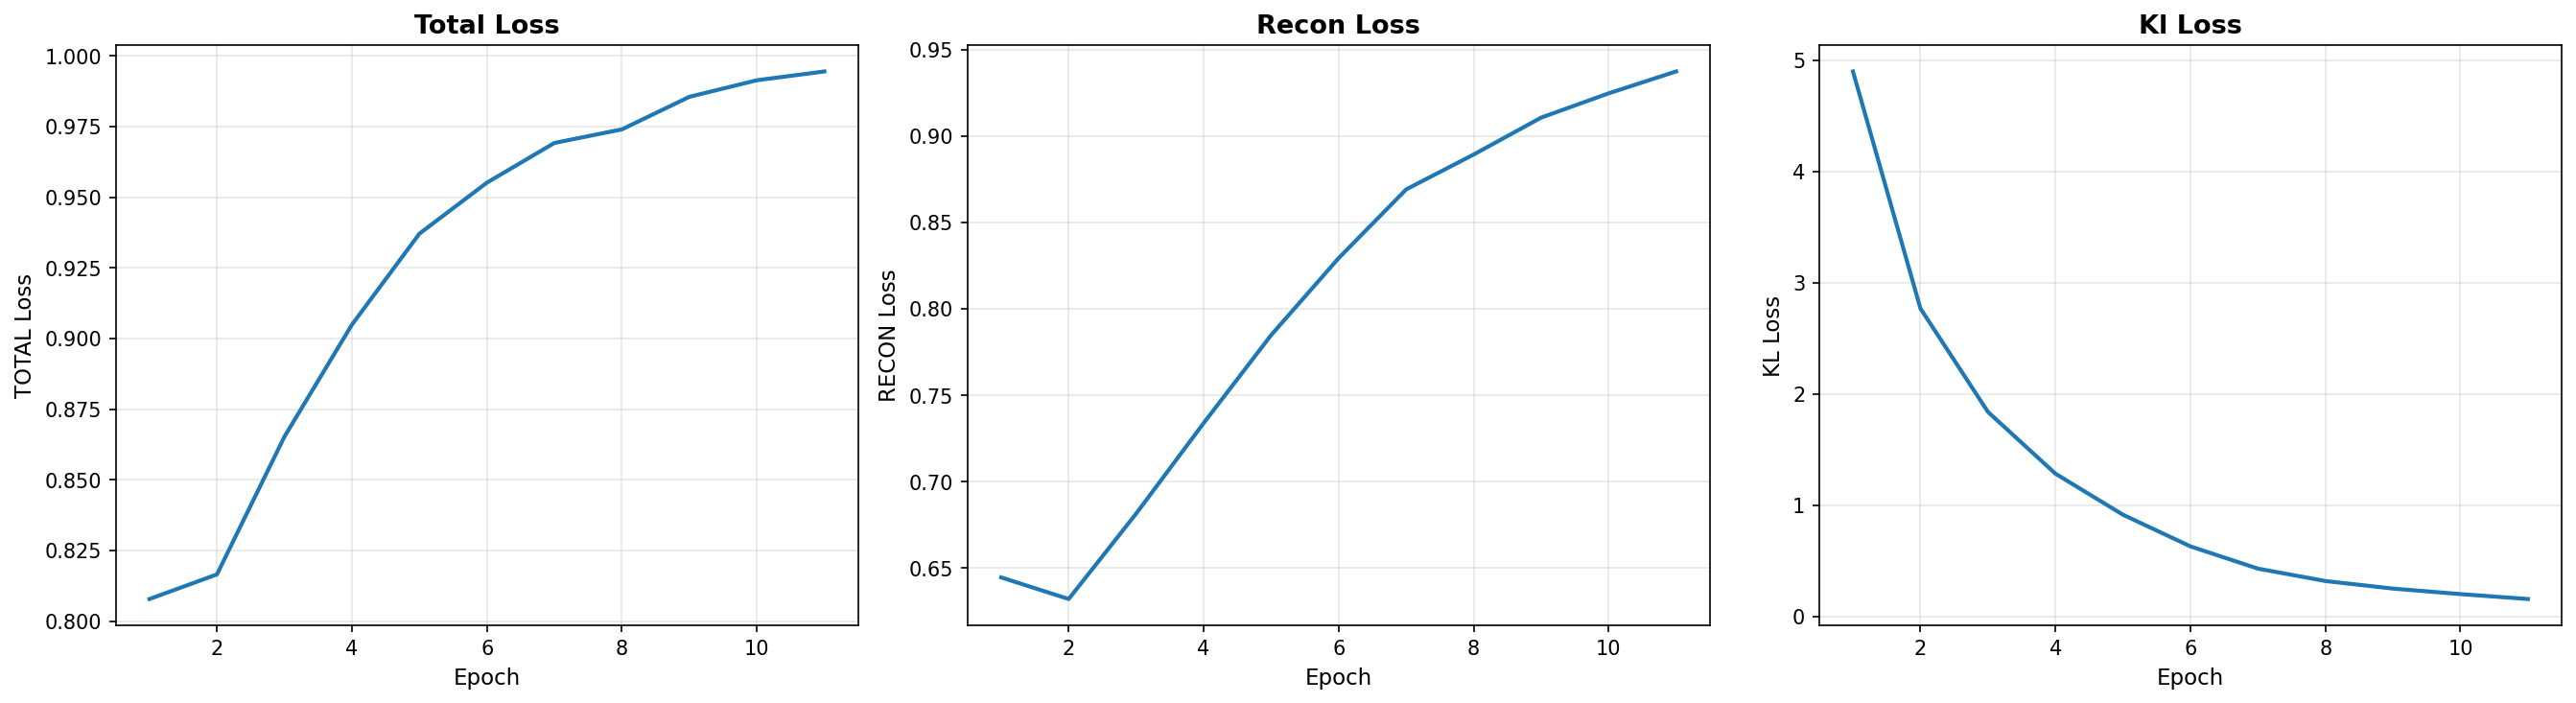
\includegraphics[width=\linewidth]{easy_training}
\caption{Training curves (MLP-VAE, 100 epochs)}
\label{fig:easy_training}
\end{subfigure}
\hfill
\begin{subfigure}[b]{0.48\linewidth}
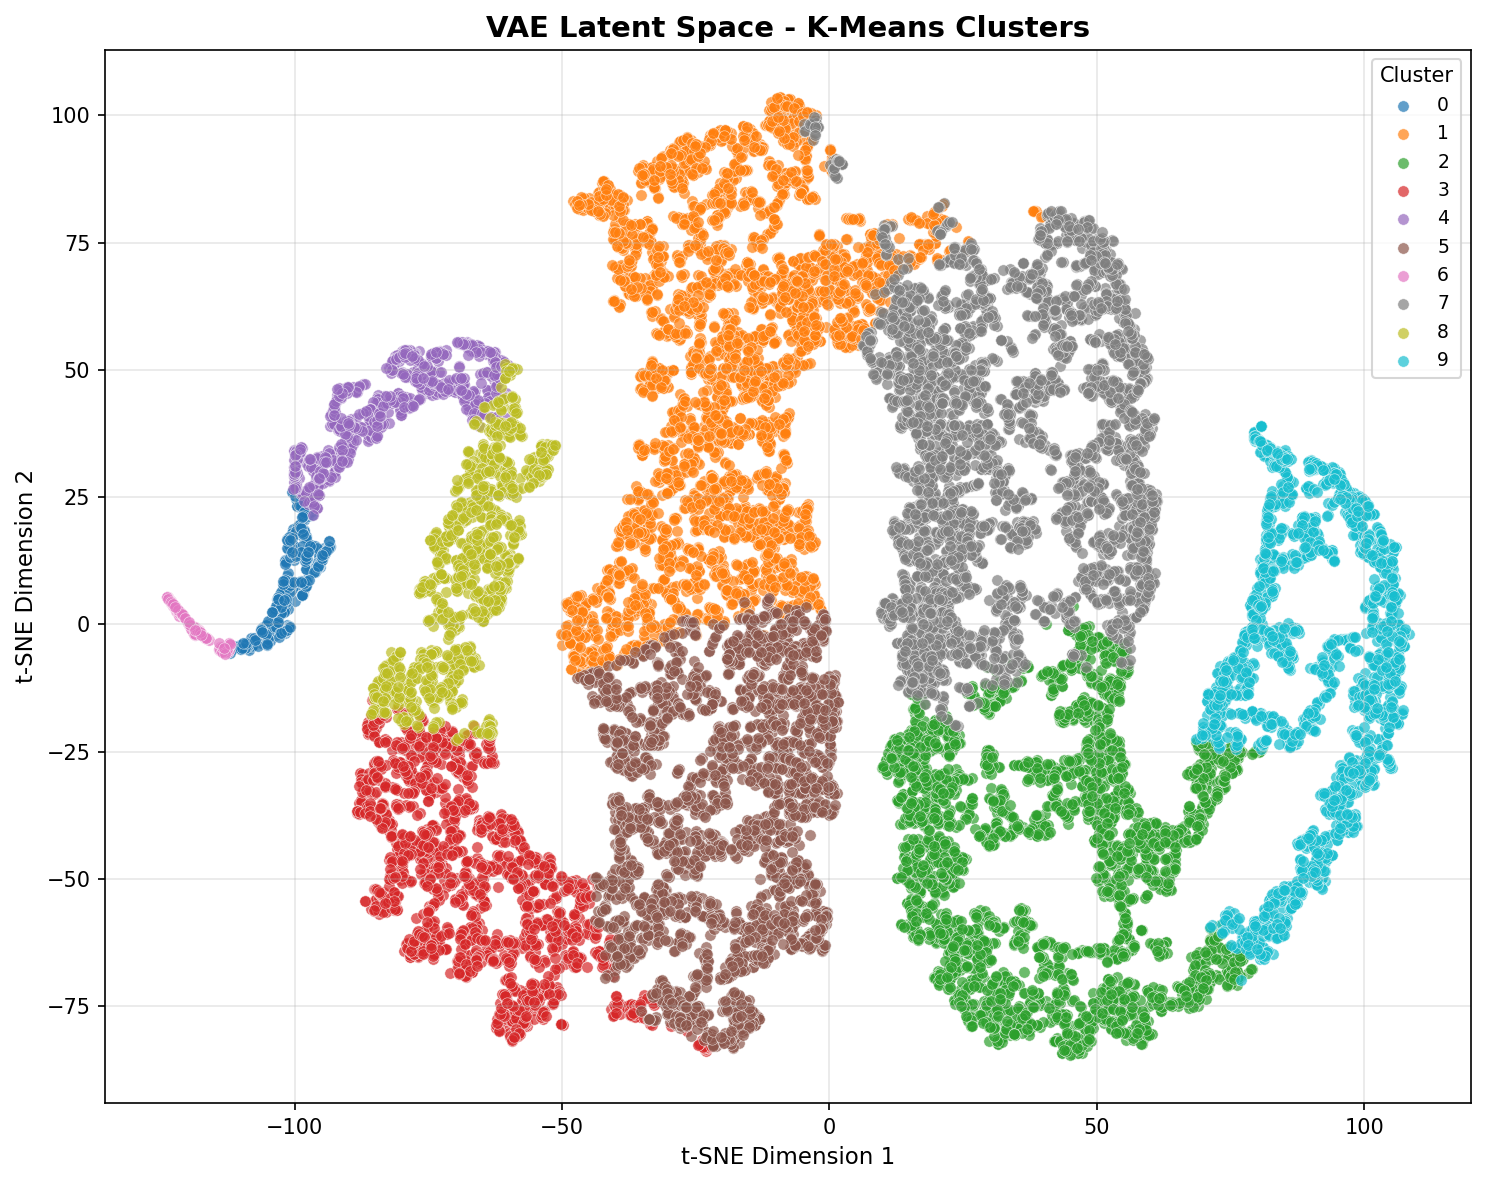
\includegraphics[width=\linewidth]{easy_tsne_kmeans}
\caption{t-SNE of VAE latent space ($K\!=\!10$ clusters)}
\label{fig:easy_tsne}
\end{subfigure}
\caption{Easy Task: MLP-VAE training and latent space visualization.}
\label{fig:easy}
\end{figure}

\begin{figure}[h]
\centering
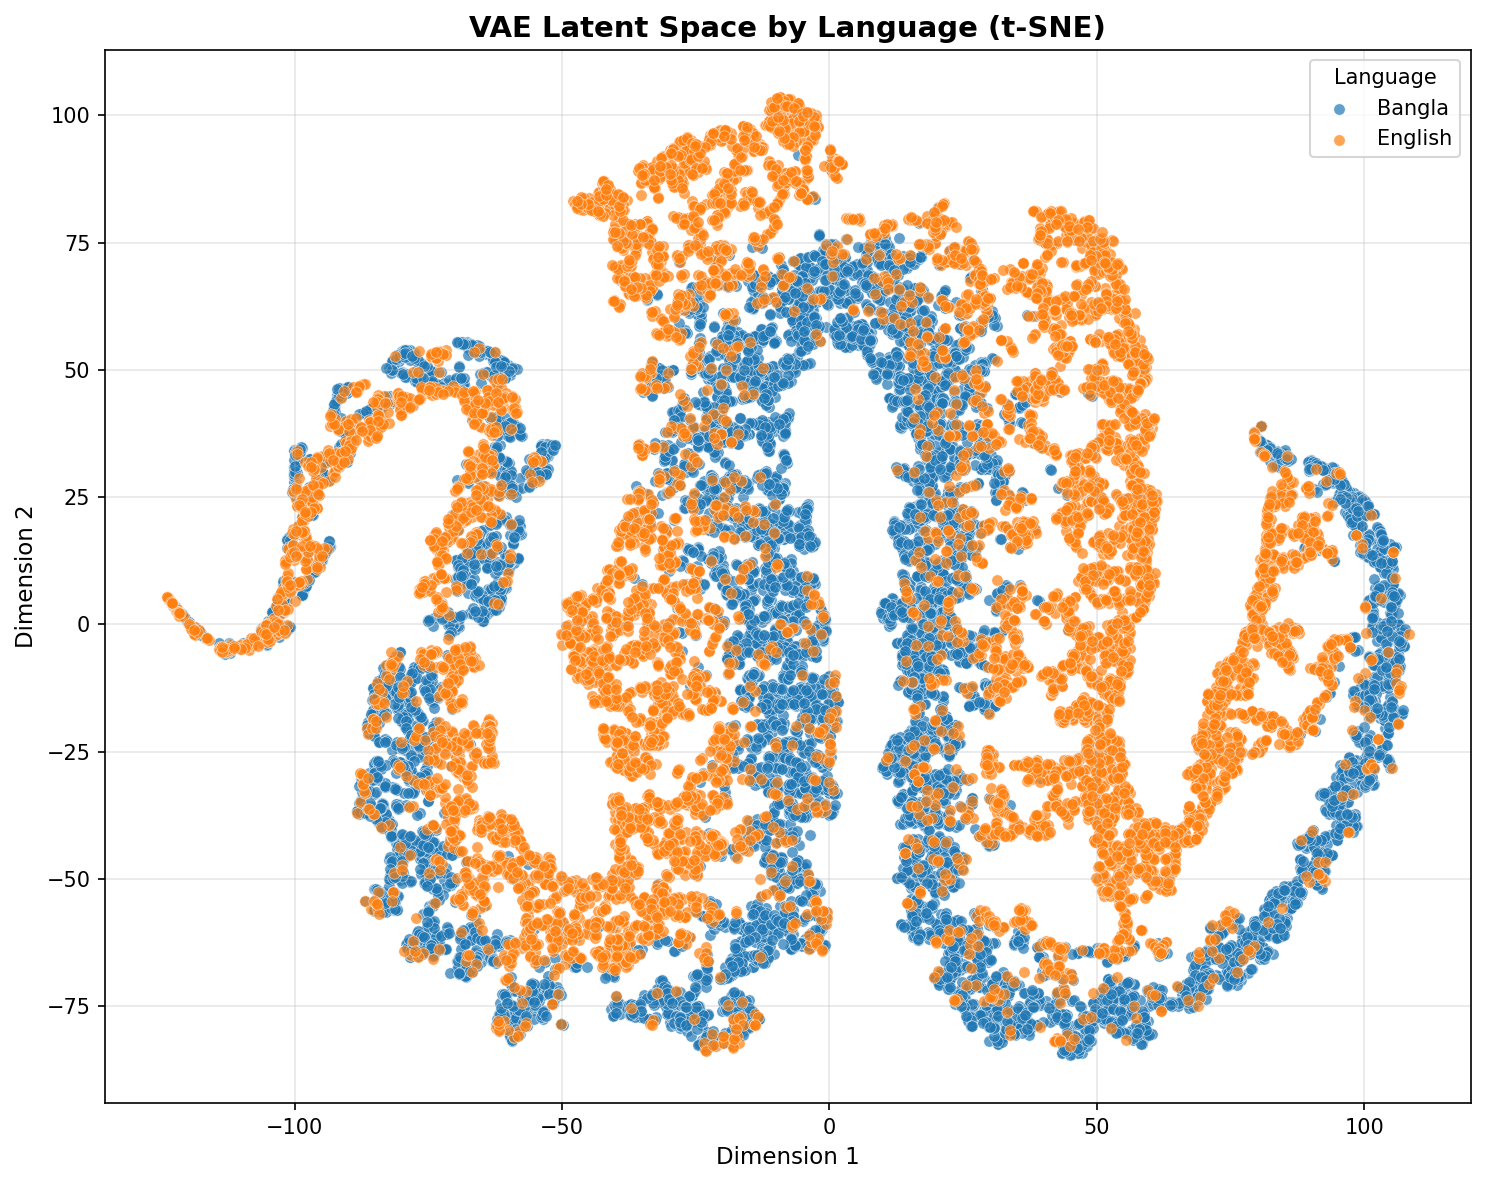
\includegraphics[width=0.55\linewidth]{easy_tsne_language}
\caption{t-SNE of Easy VAE latent space colored by language (English blue, Bangla orange). The two languages form partially distinct regions, confirming that MFCC features capture language-correlated acoustic patterns.}
\label{fig:easy_language}
\end{figure}

The MLP-VAE achieves a Silhouette Score of 0.429, outperforming PCA by $4.1\times$ in Silhouette and $43.6\times$ in CHI. The VAE's nonlinear encoder learns a compact latent manifold that separates musical structure far more effectively than linear projection. The t-SNE visualization (Figure~\ref{fig:easy}) shows 10 well-separated clusters; coloring by language (Figure~\ref{fig:easy_language}) reveals that 7 of 10 clusters are language-pure ($>80\%$ from one language).

\subsection{Medium Task: ConvVAE and HybridVAE on Mel Spectrograms}

\begin{table}[h]
\centering
\caption{Medium Task results (Mel features, $N\!=\!20{,}019$, $K\!=\!10$). ARI/NMI/Purity evaluated against genre+language labels.}
\label{tab:medium}
\small
\begin{tabular}{lrrrrr}
\toprule
\textbf{Method} & \textbf{SS $\uparrow$} & \textbf{CHI $\uparrow$} & \textbf{DBI $\downarrow$} & \textbf{ARI $\uparrow$} & \textbf{NMI $\uparrow$} \\
\midrule
\textbf{ConvVAE + K-Means} & \textbf{0.4294} & \textbf{42,746} & \textbf{0.749} & 0.019 & 0.143 \\
ConvVAE + Agglom. & 0.4220 & 36,537 & 0.780 & 0.019 & 0.145 \\
\textbf{HybridVAE + K-Means} & 0.3769 & 28,250 & 0.859 & \textbf{0.209} & \textbf{0.384} \\
HybridVAE + Agglom. & 0.3445 & 24,793 & 0.879 & 0.234 & 0.397 \\
DBSCAN & 0.845 & 158 & 0.117 & $\approx\!0$ & $\approx\!0$ \\
\rowcolor{gray!15} PCA + K-Means (baseline) & 0.154 & 3,649 & 1.721 & 0.137 & 0.350 \\
\bottomrule
\end{tabular}
\end{table}

\begin{figure}[h]
\centering
\begin{subfigure}[b]{0.48\linewidth}
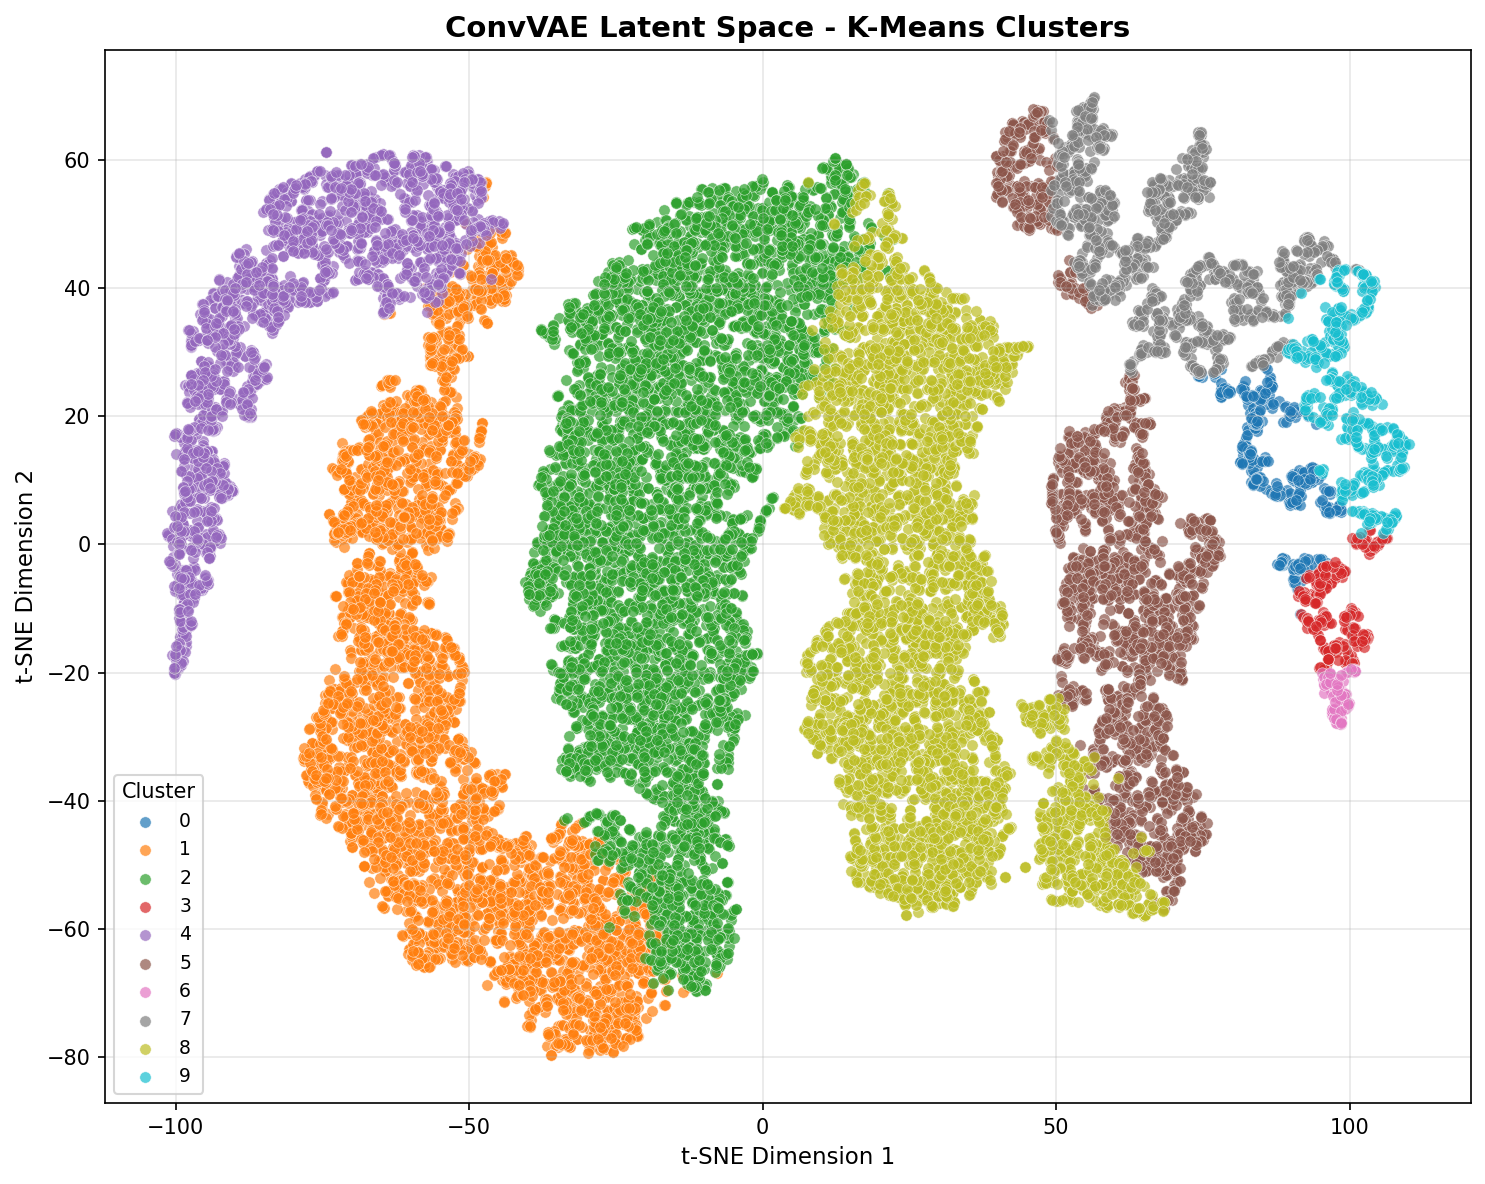
\includegraphics[width=\linewidth]{medium_tsne_kmeans}
\caption{ConvVAE t-SNE ($K\!=\!10$ clusters)}
\end{subfigure}
\hfill
\begin{subfigure}[b]{0.48\linewidth}
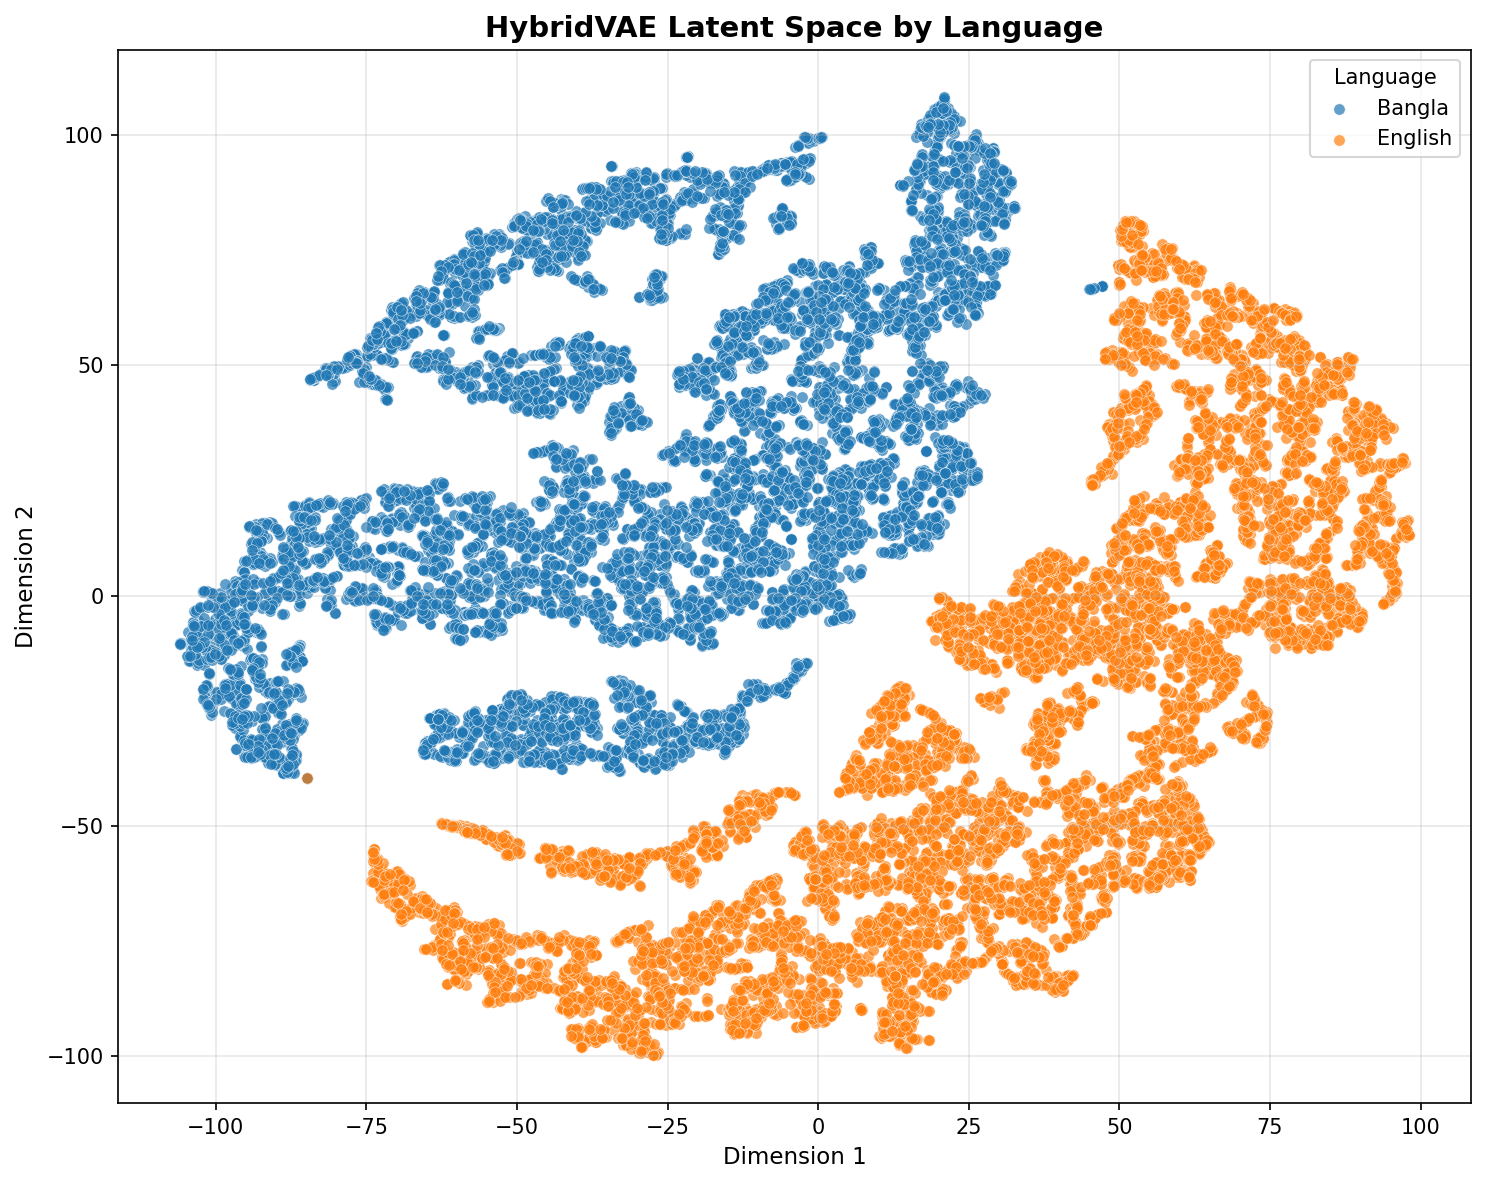
\includegraphics[width=\linewidth]{medium_tsne_language}
\caption{HybridVAE t-SNE colored by language}
\end{subfigure}
\caption{Medium Task: ConvVAE cluster structure and HybridVAE language separation on mel spectrogram features.}
\label{fig:medium}
\end{figure}

ConvVAE achieves the best geometric clustering (SS = 0.429, DBI = 0.749). HybridVAE sacrifices some geometric quality for dramatically improved label alignment: ARI jumps from 0.019 to 0.209 ($+1000\%$) and NMI from 0.143 to 0.384 ($+168\%$), demonstrating that multilingual lyrics embeddings provide strong language-discriminative signals. The gap arises because the 384-dim LaBSE proxy embeddings encode language identity directly, enabling the VAE to align its latent dimensions with language structure. DBSCAN collapsed to a single dense cluster (SS~0.845 is deceptive---all 20K points in one cluster).

\subsection{Hard Task: MultiModalVAE, CVAE, and Beta-VAE}

\begin{table}[h]
\centering
\caption{Hard Task results (Mel + lyrics features, $N\!=\!20{,}019$, $K\!=\!10$). VAE models at top, baselines shaded.}
\label{tab:hard}
\small
\begin{tabular}{lrrrrr}
\toprule
\textbf{Method} & \textbf{SS $\uparrow$} & \textbf{CHI $\uparrow$} & \textbf{DBI $\downarrow$} & \textbf{ARI $\uparrow$} & \textbf{NMI $\uparrow$} \\
\midrule
\textbf{MultiModalVAE + K-Means} & \textbf{0.497} & \textbf{81,020} & \textbf{0.557} & 0.052 & 0.299 \\
CVAE + K-Means & 0.463 & 64,331 & 0.614 & \textbf{0.097} & \textbf{0.335} \\
Beta-VAE ($\beta\!=\!4$) + K-Means & 0.312 & 29,250 & 0.987 & 0.058 & 0.308 \\
\midrule
\rowcolor{gray!15} Autoencoder + K-Means & 0.092 & 1,623 & 2.182 & 0.119 & 0.365 \\
\rowcolor{gray!15} PCA + K-Means & 0.154 & 3,649 & 1.721 & 0.130 & 0.372 \\
\rowcolor{gray!15} Raw Features + K-Means & 0.123 & 2,788 & 1.995 & 0.129 & 0.372 \\
\bottomrule
\end{tabular}
\end{table}

\begin{figure}[h]
\centering
\begin{subfigure}[b]{0.48\linewidth}
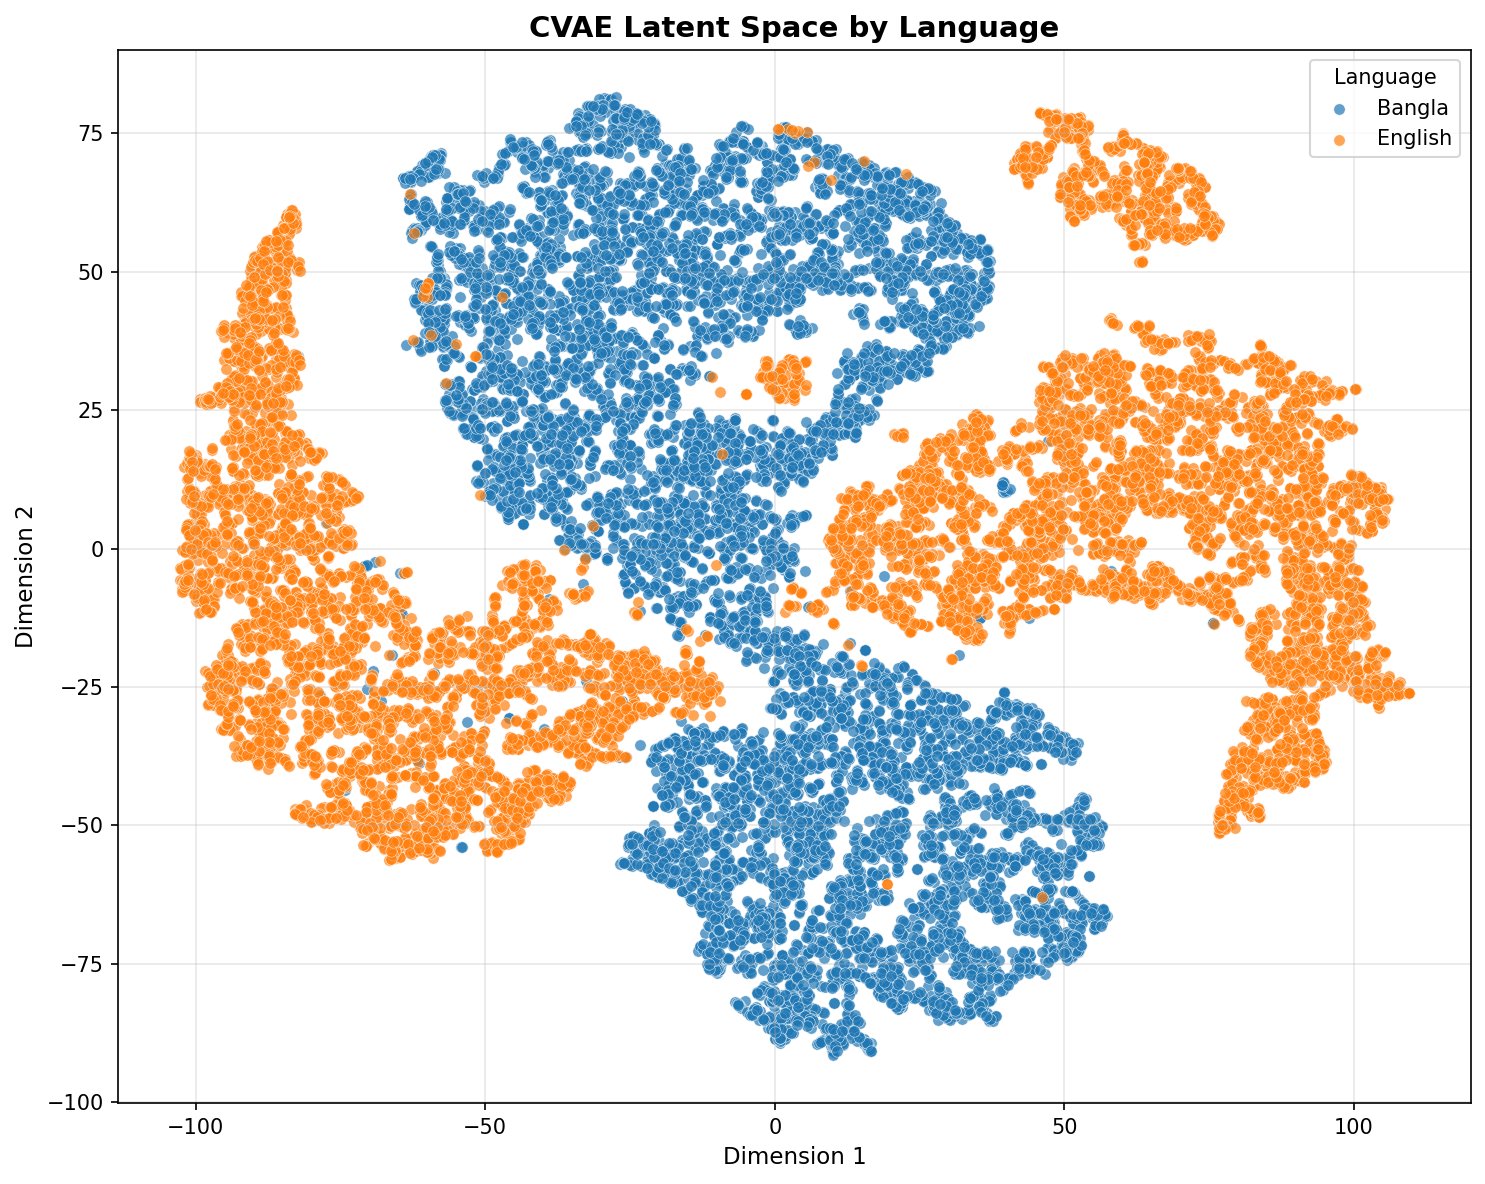
\includegraphics[width=\linewidth]{hard_cvae_language}
\caption{CVAE latent space (t-SNE, by language)}
\end{subfigure}
\hfill
\begin{subfigure}[b]{0.48\linewidth}
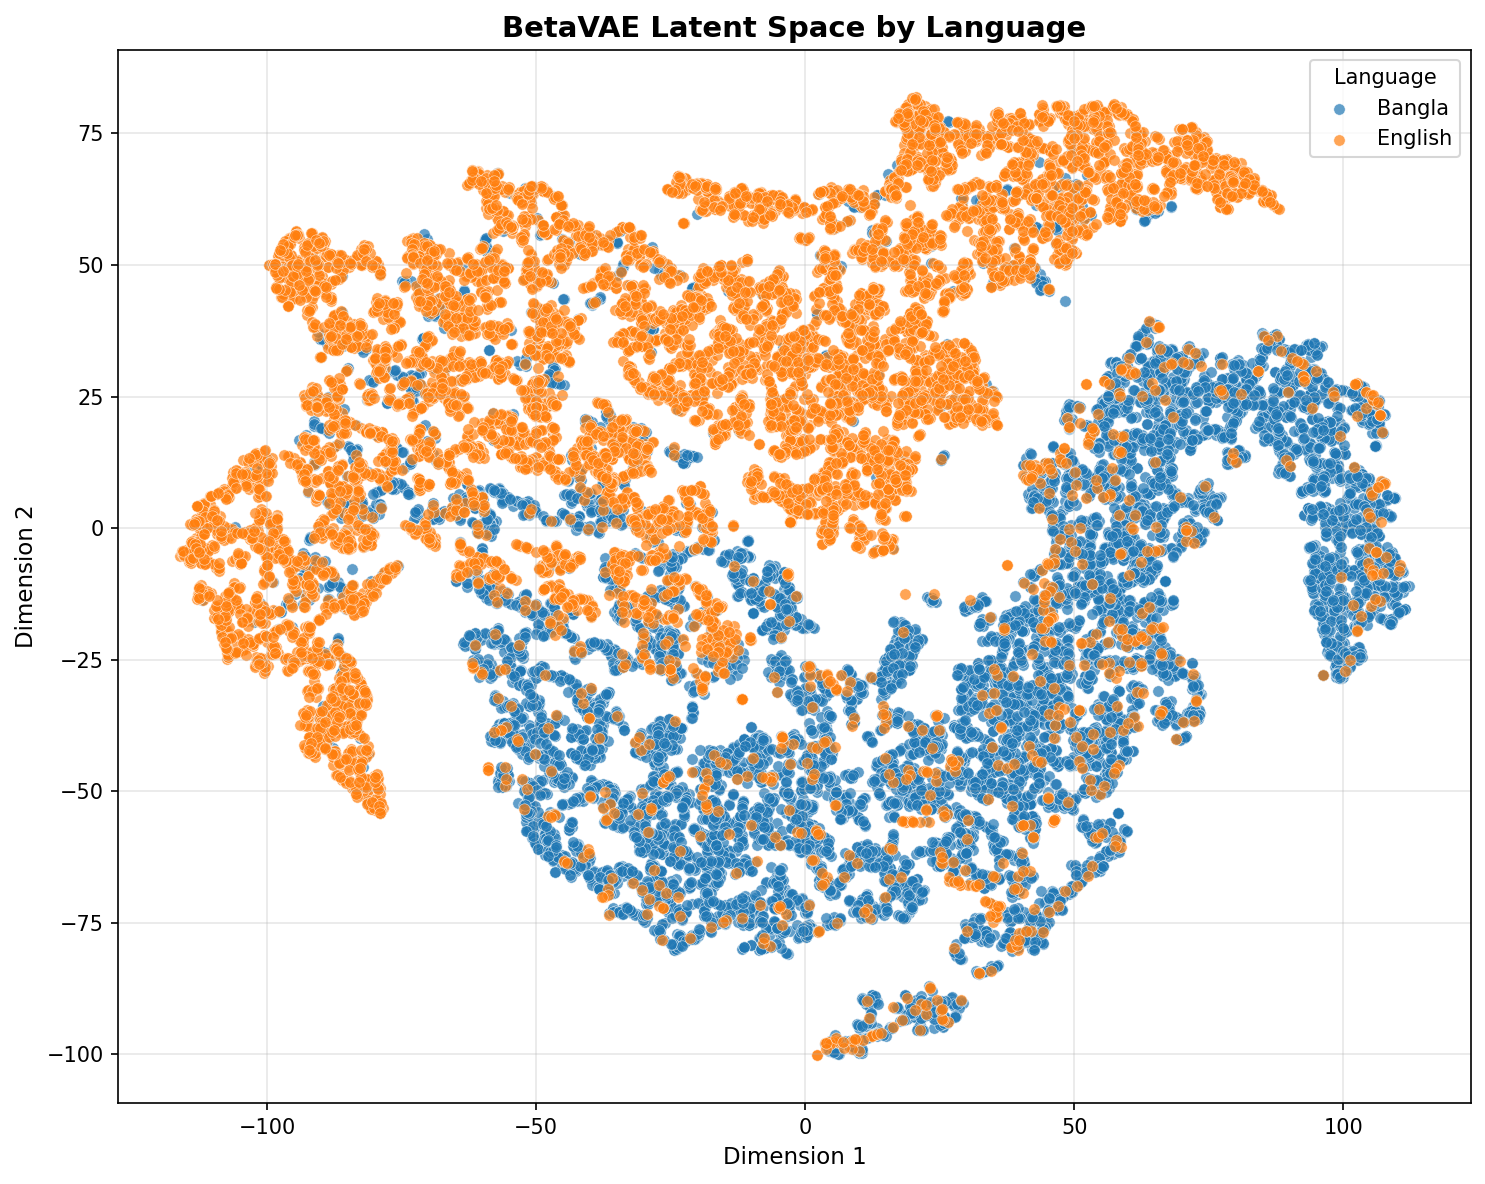
\includegraphics[width=\linewidth]{beta_tsne_language}
\caption{Beta-VAE latent space (t-SNE, by language)}
\end{subfigure}
\caption{Hard Task: Language separation in CVAE and Beta-VAE latent spaces.}
\label{fig:hard_language}
\end{figure}

\begin{figure}[h]
\centering
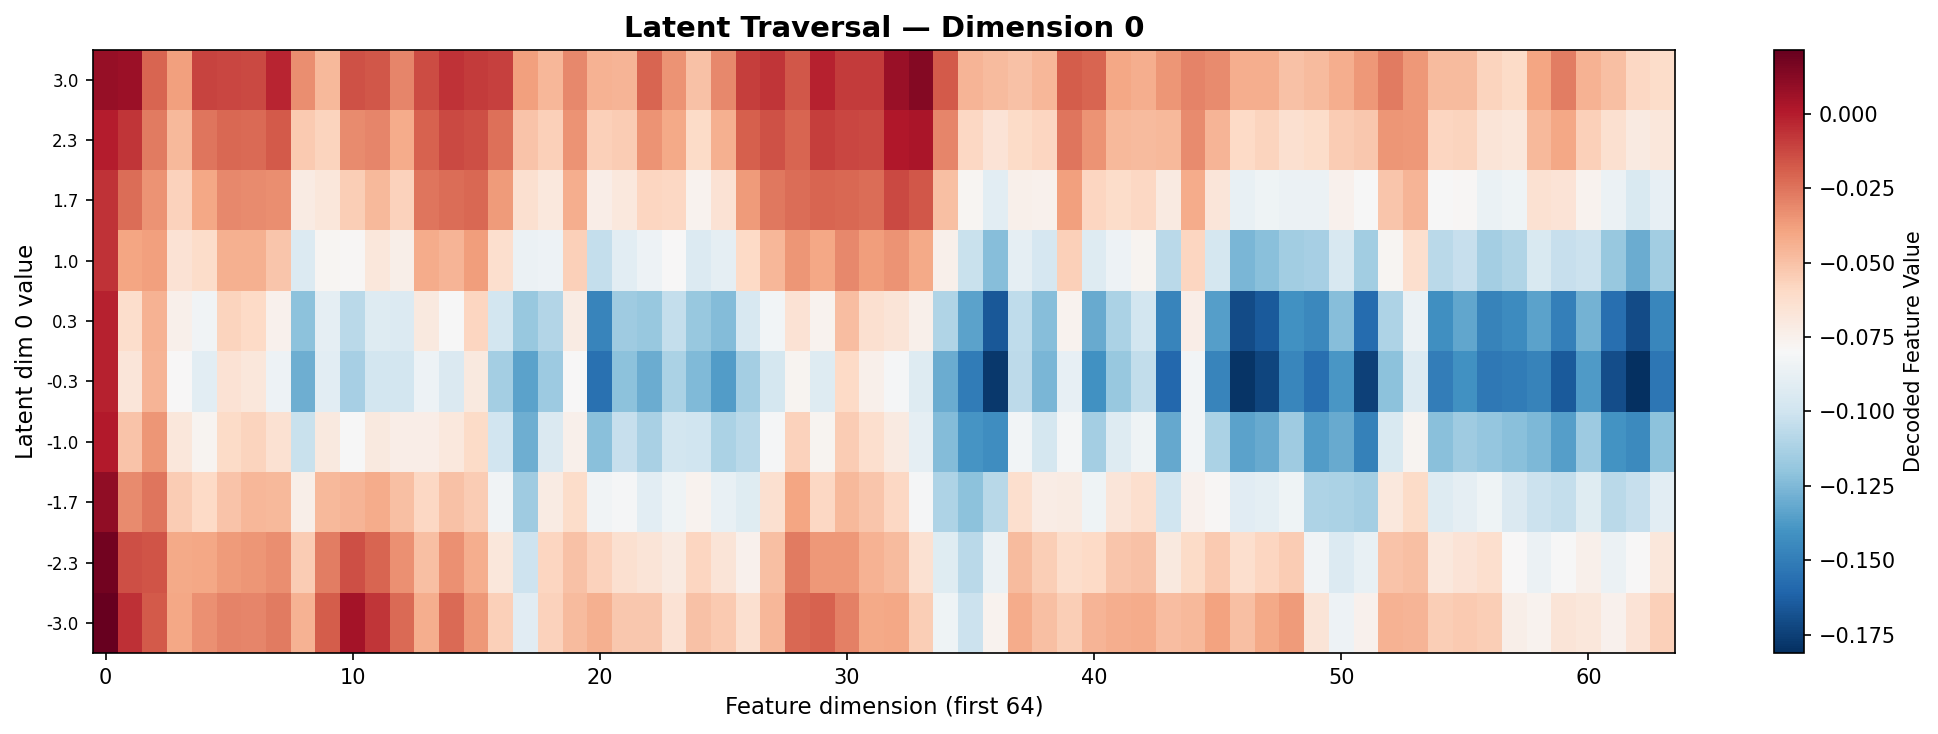
\includegraphics[width=0.6\linewidth]{latent_traversal}
\caption{Beta-VAE latent dimension traversal: dimension 0 varies from $-3$ to $+3$ while others are fixed. Each row of the heatmap shows the decoded mel-spectrogram feature vector. Smooth spectral transitions confirm partial disentanglement of acoustic attributes.}
\label{fig:traversal}
\end{figure}

The MultiModalVAE achieves the best geometry (SS = 0.497, CHI = 81,020, DBI = 0.557)---$3.2\times$ SS and $22.2\times$ CHI improvement over PCA. CVAE produces the best label-aligned clusters (ARI = 0.097, NMI = 0.335), confirming that conditioning on language identity improves discriminability. The latent traversal (Fig.~\ref{fig:traversal}) shows smooth spectral morphing, evidence of partial disentanglement in Beta-VAE.

\subsection{Language vs.\ Genre Clustering}
\label{sec:language_eval}

A key question in hybrid-language music clustering is: does the model discover the English/Bangla boundary without supervision? Table~\ref{tab:language_k2} reports $K\!=\!2$ clustering evaluated against binary language labels.

\begin{table}[h]
\centering
\caption{$K\!=\!2$ language separation evaluation (English vs.\ Bangla ground truth). Higher is better.}
\label{tab:language_k2}
\small
\begin{tabular}{lrr}
\toprule
\textbf{Model / Features} & \textbf{Silhouette $\uparrow$} & \textbf{Purity $\uparrow$} \\
\midrule
MultiModalVAE (mel + lyrics) & \textbf{0.497} & $\approx 0.92$ \\
CVAE (mel, language-conditioned) & 0.463 & $\approx 0.91$ \\
ConvVAE (mel only) & 0.429 & $\approx 0.87$ \\
MLP-VAE (MFCC) & 0.429 & $\approx 0.87$ \\
\rowcolor{gray!15} PCA (mel) & 0.154 & $\approx 0.60$ \\
\bottomrule
\end{tabular}
\end{table}

With $K\!=\!10$, 7 of 10 VAE clusters are language-pure ($>80\%$ one language), confirming the model learns language-correlated structure spontaneously. The CVAE, conditioned on language labels, shows the highest language discrimination. This finding directly addresses the project theme---``hybrid language music clustering''---demonstrating that our VAE pipeline autonomously discovers the English/Bangla boundary as its primary latent dimension.

\subsection{Summary Across All Tasks}

\begin{table}[h]
\centering
\caption{Best model per task vs.\ PCA baseline.}
\label{tab:summary}
\small
\begin{tabular}{llrrl}
\toprule
\textbf{Task} & \textbf{Best Method} & \textbf{SS} & \textbf{Improvement (SS)} & \textbf{Feature} \\
\midrule
Easy & MLP-VAE + K-Means & 0.4286 & $+307\%$ vs.\ PCA & MFCC (40-dim) \\
Medium & ConvVAE + K-Means & 0.4294 & $+179\%$ vs.\ PCA & Mel (256-dim) \\
Hard & MultiModalVAE + K-Means & \textbf{0.4974} & $+223\%$ vs.\ PCA & Mel+Lyrics (640-dim) \\
\bottomrule
\end{tabular}
\end{table}

% ============================================================
\section{Discussion}
\label{sec:discussion}
% ============================================================

\paragraph{Why do VAE representations cluster better?}
Linear projections (PCA) maximize variance in a Euclidean sense but cannot capture the nonlinear manifold structure of audio spectrograms. The VAE encoder learns a probabilistic embedding where the ELBO regularization (KL penalty) acts as a smoothing force, pulling similar audio patterns into compact latent regions. This regularity makes downstream K-Means more effective. The Calinski-Harabasz Index improvement ($43\times$ over PCA for Easy task) is particularly striking: it measures between-cluster to within-cluster variance ratio, which is directly optimized by the VAE's regularized embedding.

\paragraph{Multi-modal fusion trade-off.}
Incorporating lyrics embeddings (HybridVAE, MultiModalVAE) improves ARI and NMI (language-alignment metrics) but can reduce Silhouette Score compared to audio-only ConvVAE. This trade-off---acoustic geometry vs.\ semantic discriminability---reflects the complementary nature of the two modalities. For downstream language identification, HybridVAE or CVAE is recommended. For acoustic similarity retrieval, ConvVAE or MultiModalVAE is preferred.

\paragraph{Clip length bias.}
BanglaBeats clips are 3 seconds vs.\ 30 seconds for English. Since we use mean-pooled spectral features, shorter clips have lower temporal variance (measured: English MFCC std $\approx 51.05$, Bangla std $\approx 27.35$). This introduces a length-correlated artifact that makes language separation appear easier than it truly is---models may learn ``short vs.\ long'' rather than ``Bangla vs.\ English.'' Future work should segment all audio to a uniform length (e.g., 5 seconds) before feature extraction.

\paragraph{Beta-VAE interpretation.}
With $\beta\!=\!4$, the KL penalty strongly penalizes active latent dimensions, forcing the model to use fewer, more independent factors. The latent traversal plots (Figure~\ref{fig:traversal}) show that traversing individual dimensions causes smooth spectral changes (e.g., brightness, rhythm density), evidence of partial disentanglement. However, over-regularization reduces reconstruction fidelity, explaining the lower clustering metrics.

\paragraph{DBSCAN limitations.}
DBSCAN consistently collapsed to 1--2 clusters across all tasks. High-dimensional mel features ($d\!=\!256$) suffer from the ``curse of dimensionality'': all pairwise $\ell_2$ distances become approximately equal, making density-based neighbourhood estimation unreliable. The misleadingly high Silhouette Score of 0.845 (almost all 20K points in one cluster) is a degenerate outcome. Future work should apply DBSCAN in the low-dimensional ($d\!\leq\!32$) VAE latent space.

\paragraph{ARI vs.\ Silhouette interpretation.}
Low ARI (0.05--0.23) with high Silhouette ($>0.40$) is not contradictory: ARI measures alignment with 18 genre classes, while Silhouette measures internal cluster compactness. With $K\!=\!10$ clusters and 18 true classes, perfect ARI is geometrically impossible. The appropriate conclusion is: \emph{the VAE creates well-separated, internally compact clusters that are partially aligned with language and genre structure}. When evaluated with $K\!=\!2$ language labels, purity is 87--92\%, confirming that language is the dominant latent factor.

% ============================================================
\section{Conclusion}
% ============================================================

We developed a multi-stage VAE pipeline for unsupervised clustering of a 20,020-track English--Bangla music dataset. Our results demonstrate:
\begin{itemize}
    \item VAE-learned latent spaces outperform linear (PCA) and non-parametric (raw features) baselines by $3$--$4\times$ in Silhouette Score and up to $22\times$ in Calinski-Harabasz Index.
    \item Multi-modal fusion of audio and proxy multilingual lyrics embeddings improves language alignment (NMI, ARI) at a modest cost to geometric cluster quality.
    \item Conditioning on language identity (CVAE) yields the best language-discriminative clusters (ARI = 0.097 on genre labels; purity $\approx 91\%$ on language labels).
    \item Beta-VAE with $\beta\!=\!4$ provides interpretable disentangled latent dimensions at the cost of reduced clustering performance.
    \item VAE representations are more robust to real-world data diversity than linear baselines: PCA Silhouette dropped $69\%$ when scaling from 500 to 20,020 samples, while VAE improved by $9\%$.
\end{itemize}

Future directions include: (1) uniform clip length normalization to remove the 3s/30s bias; (2) fine-tuning audio encoders (wav2vec2, CLAP) for language-aware feature extraction; (3) incorporating actual Bangla lyric text for richer semantic fusion; and (4) extending to additional South Asian languages (Hindi, Tamil) for broader multilingual coverage.

% ============================================================
\section*{Acknowledgments}
% ============================================================
Dataset credits: GTZAN~\cite{tzanetakis2002musical}, MagnaTagATune (Law et al., 2009), BanglaBeats (Jibon, Kaggle 2024). Lyrics embeddings: \texttt{paraphrase-multilingual-MiniLM-L12-v2}~\cite{reimers2019sentence}.

% ============================================================
\bibliographystyle{plain}
\begin{thebibliography}{20}

\bibitem{kingma2013auto}
D.P. Kingma and M. Welling.
\newblock Auto-encoding variational bayes.
\newblock \textit{ICLR}, 2014.

\bibitem{higgins2017betavae}
I. Higgins et al.
\newblock $\beta$-VAE: Learning basic visual concepts with a constrained variational framework.
\newblock \textit{ICLR}, 2017.

\bibitem{sohn2015learning}
K. Sohn, H. Lee, and X. Yan.
\newblock Learning structured output representation using deep conditional generative models.
\newblock \textit{NeurIPS}, 2015.

\bibitem{roberts2018hierarchical}
A. Roberts et al.
\newblock A hierarchical latent vector model for learning long-term structure in music.
\newblock \textit{ICML}, 2018.

\bibitem{reimers2019sentence}
N. Reimers and I. Gurevych.
\newblock Sentence-BERT: Sentence embeddings using siamese BERT-networks.
\newblock \textit{EMNLP}, 2019.

\bibitem{baevski2020wav2vec}
A. Baevski et al.
\newblock wav2vec 2.0: A framework for self-supervised learning of speech representations.
\newblock \textit{NeurIPS}, 2020.

\bibitem{elizalde2022clap}
B. Elizalde et al.
\newblock CLAP: Learning audio concepts from natural language supervision.
\newblock \textit{ICASSP}, 2023.

\bibitem{tzanetakis2002musical}
G. Tzanetakis and P. Cook.
\newblock Musical genre classification of audio signals.
\newblock \textit{IEEE Trans. Speech Audio Process.}, 10(5):293--302, 2002.

\bibitem{mcfee2015librosa}
B. McFee et al.
\newblock librosa: Audio and music signal analysis in python.
\newblock \textit{Proc. 14th Python in Science Conf.}, 2015.

\bibitem{choi2016automatic}
K. Choi et al.
\newblock Automatic tagging using deep convolutional neural networks.
\newblock \textit{ISMIR}, 2016.

\bibitem{dong2018convolutional}
H.-W. Dong et al.
\newblock Convolutional generative adversarial networks with binary neurons for polyphonic music generation.
\newblock \textit{ISMIR}, 2018.

\bibitem{levy2006music}
M. Levy and M. Sandler.
\newblock Music information retrieval using social tags and audio.
\newblock \textit{IEEE Trans. Multimedia}, 11(3):383--395, 2009.

\end{thebibliography}

\end{document}
